\chapter{2. opgave}
Da vi tjekkede for outliers haved vi 12 kategorier at kigge på de er skrevet nedenfor i hvor tekst er skrevet til hver, givet om der er outliers eller ej.
\begin{enumerate}
\item Patient number id. \newline
De vil ikke give mening at lave en test da det er et nummer givet til dem 
\item  Time in study time.\\
\begin{figure}[h]
    \centering
    \includegraphics[width=0.6\linewidth]{Basses_kode/Billeder_duration/Boxplot_of_ time .pdf}
\end{figure}
\textbf{Outliers: }På billedet kan de ses at der er en enkel outlier, men siden det er en person der var i live i slutning må vi konkludere at det eneste der er at se er en rask patient der kom ind i forsøget tidligt.\\
\textbf{Distribution :} Plotter man densiteten af tidsgrafen ser man en nogenlunde normalfordeling dog med en, som forventet, tung højre hale


\item Cause of death status. \newline
Dette kan vi ikke rigtig kigge på outliers, da det er dødsårsagen 
\item Dead/alive at time of follow-up dead. \newline
Her kan vi Heller ikke kigge på outliers da det er status på patient efter et bestemt tids interval
\item Inflammatory cell infiltration score ici. \newline
Heller ikke her
\item Presence of epitheloid cells epicell. \newline
Heller ikke her
\item Presence of ulceration ulceration. \newline
Heller ikke her
\item Thickness of tumor (1/100mm) thickness.
\newline
\begin{figure}[h]
    \centering
    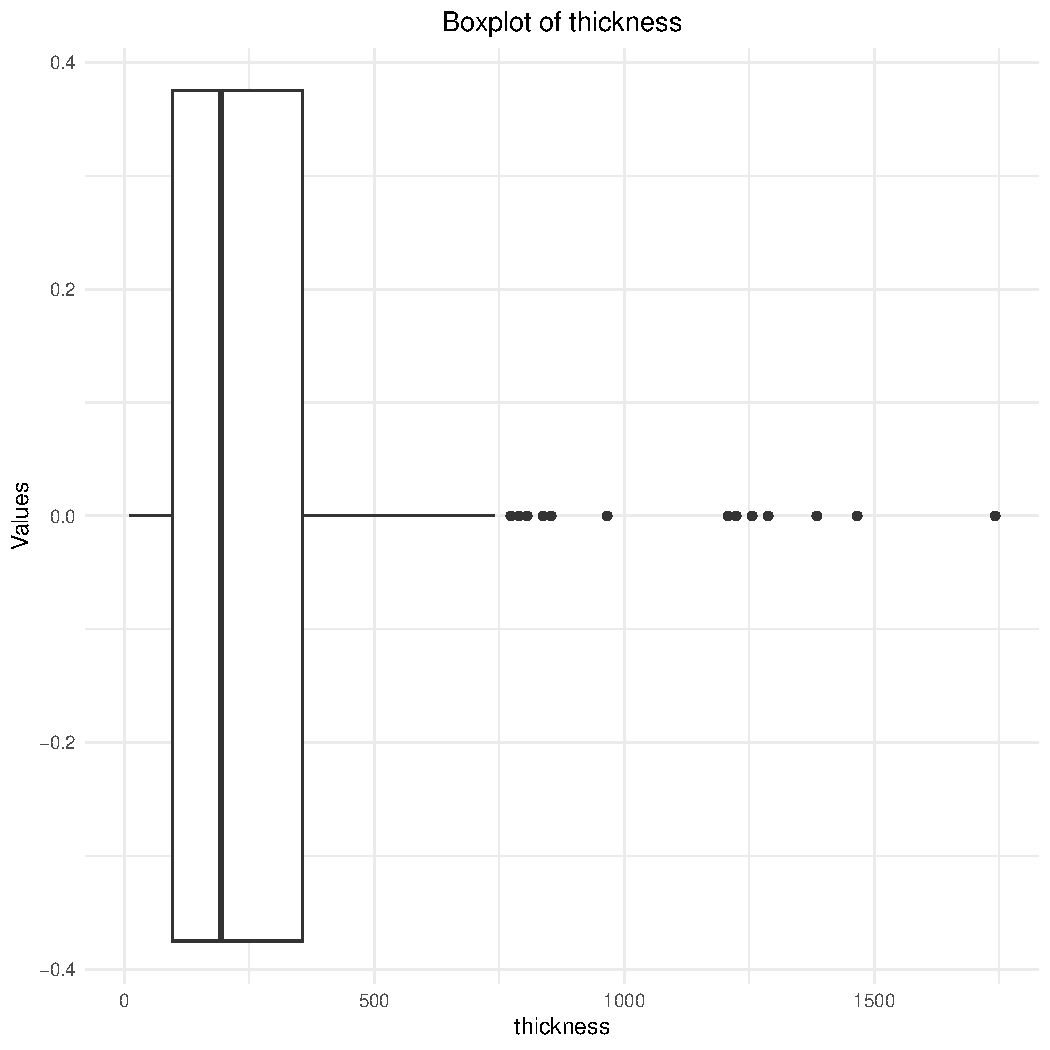
\includegraphics[width=0.5\linewidth]{Basses_kode/Billeder_duration/Boxplot_of_ thickness .pdf}
\end{figure}
\textbf{Outliers:}Selvom vi ser mange Outliers, ved vi ikke om størrelsen har indflydelse på om patienten overlever eller ej, det bliver besvaret i næste opgave\\
\textbf{Distribution: } Tykkelsen af tumor fremstår som en betadistribution som er, naturligvis, ikke negativ, stiger i starten og falder derefter og får en lang højre hale. Undersøges yderligere logaritmen til disse værdier fremgår en nogenlunde normaldistribution.\\

\item Sex sex.\\
Her kigger vi Heller ikke på outliers
\item Age at operation age.
\newline
\begin{figure}[h]
    \centering
    \includegraphics[width=0.6\linewidth]{Basses_kode/Billeder_duration/Boxplot_of_ age .pdf}
\end{figure}
\textbf{Outliers: }Her ser vi en enkelt ung outlier 
\textbf{Age: } Aldersmæssigt haves en tung venstrehale og ellers fremstår en normal distribution nogenlunde
\newpage
\item Natural log of thickness/100 logthick.
\newline
\begin{figure}[h]
    \centering
    \includegraphics[width=0.6\linewidth]{Basses_kode/Billeder_duration/Boxplot_of_ logthick .pdf}
\end{figure}
\textbf{Outliers: }We see one outlier when taking log to it but to dertemin if the outlier has any influence on the health of the patient another method must be used aswell\\
\textbf{Distribution: }Kigges på distributionen af logaritmen af tykkelsen på tumor, vil der være en nogenlunde normaldistribution, dog med en tung venstre hale.
\item Depth of invasion of tumor score invas2.
\end{enumerate}

Med henblik på de resterende, ikke kontinuerte variable, er der en fin distribution kategorierne imellem.



\chapter{3. Opgave}
